%Note di Ingegneria del Software
%Sommario: Gestione progetto, Tempo calendario/risorsa, Ruoli, Pianificazione, Gantt, PERT, WBS, Problemi allocazione risorse, CoCoMo, Piano di progetto e rischi

\cornell{Gestione Progetto}{Insieme di attività (precisamente è un processo: project management) che governa tutto ciò che facciamo nel progetto.\\
Appartiene alla categoria dei processi organizzativi.}
\cornell{Tempo di Calendario VS Tempo come risorsa}{Questi due "tempi" sono molto diversi, mentre il tempo di calendario è semplice da calcolare, il tempo come risorsa dipende fortemente dalla pianificazione (un esempio è il tempo-persona)}
\cornell{Funzione Aziendale}{Una funzione permanente, indipendente dal progetto in corso di svolgimento}
\cornell{Ruolo Di Progetto}{Funzione aziendale assegnata a progetto}
\cornell{Ruoli principali}{\begin{description}
\item [Sviluppo] Responsabilità tecnica e realizzativa
\item[Direzione] Responsabilità decisionale
\item [Amministrazione] Responsabilità nella gestione di tecnologie di supporto ai processi
\item [Qualità]
\end{description}}
\cornell{Ruoli a Progetto: Analisti}{Si occupano di capire il problema.\\
Deve fare molte attività per chiarire lo scopo del progetto, quindi ha molta influenza sul successo di quest'ultimo.\\
Generalmente sono pochi, e raramente seguono il progetto fino alla fine}

\cornell{Ruoli a Progetto: Progettisti}{Si occupano dell'aspetto tecnico della soluzione dei problemi spiegati dagli analisti.\\
Definisce la miglior soluzione in termini di efficienza ed efficacia.\\
Solitamente sono pochi ed accompagnano il progetto fino alla fine.}

\cornell{Ruoli a Progetto: Programmatori}{Eseguono ciò che è stato definito dai progettisti e nulla di più.\\
Hanno competenze, visione e responsabilità molto circoscritte.\\
Sono molti.}

\cornell{Ruoli a Progetto: Verificatori}{Si occupano della verifica di conformità del progetto.\\
Durano per l'intera durata di quest'ultimo.}

\cornell{Ruoli a progetto: Responsabile}{Accentra le responsabilità di scelta ed approvazione.\\
Dura tanto quanto il progetto.\\
Ha responsabilità di: \begin{itemize}
\item Pianificazione
\item Gestione delle risorse umane
\item Controllo, coordinamento e relazioni esterne
\item Valutare richi, scelte ed alternative.
\end{itemize}}
\cornell{Ruoli a Progetto: Amministratore}{Ruolo di supporto (conosciuto anche come SysAdmin)\\
Ha il controllo dell'ambiente di lavoro.}
\cornell{Ruoli a Progetto: Gestione Qualità}{Ha una propria "way of working", quindi non cambia da progetto a progetto $ \Longrightarrow $ Funzione aziendale.\\
Ha lo scopo di massimizzare efficienza ed efficacia.}

\cornell{Pianificazione}{Organizzare il tempo di calendario assegnandoli ad attività e persone.\\
Viene fatta tramite appositi strumenti (e non su carta): \begin{itemize}
\item Diagrammi di Gantt
\item PERT/CPM
\item WBS
\end{itemize}\\
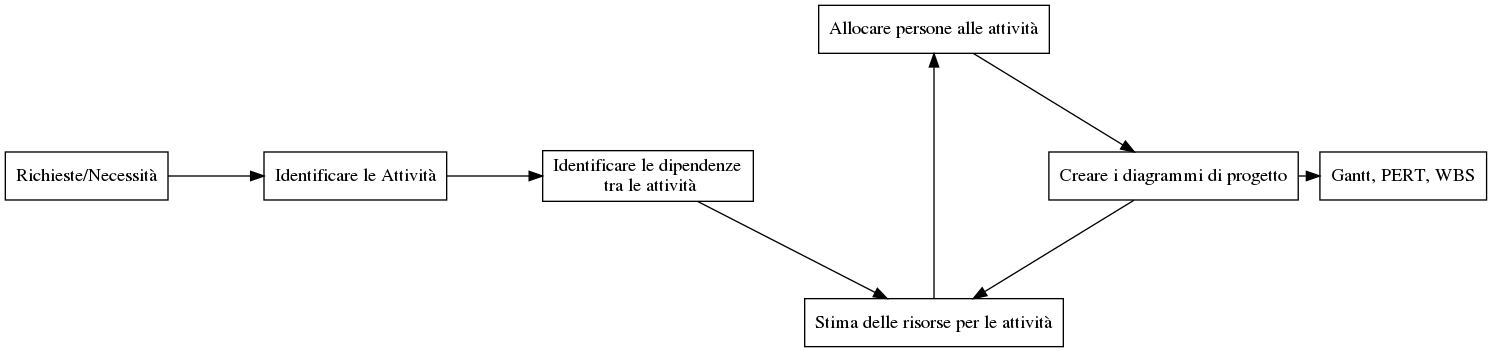
\includegraphics[scale=0.2]{images/6.png}}
\cornell{Diagrammi di GANTT}{Il diagramma di Gantt (H.L. Gantt - 1917) è un diagramma di supporto alla gestione dei progetti, esso è costituito da un asse orizzontale, che rappresenta il tempo totale del progetto, suddiviso in fasi incrementali (giorni/settimane/mesi) e da un asse verticale che rappresenta le attività di progetto.\\
Vi sono poi delle barre orizzontali che rappresentano visivamente le sequenze, la durata e l'arco temporale di ogni attività del progetto, dando l'idea di quante attività in parallelo si stanno svolgendo ed eventualmente i punti in cui la parallelizzazione è migliorabile.\\
Man mano che il progetto prosegue, vi possono essere delle barre secondarie atte a rappresentare attività sottostanti.\\
Questo diagramma però non tiene conto dell'eventuale interdipendenza di attività che dovranno essere rappresentate in altro modo.\\
Inoltre è possibile sovrapporre le barre, in modo da avere visivamente sotto mano la differenza tra la durata pianificata e la durata effettiva del progetto.\\
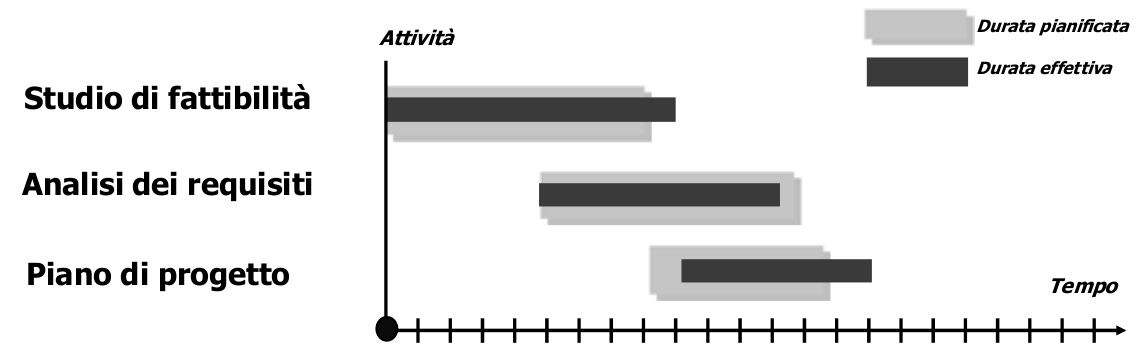
\includegraphics[scale=0.25]{images/7.png}}

\cornell{PERT/CPM}{Il PERT (Program Evaluation and Review Technique), conosciuto anche come stima a tre valori, è un metodo statistico per determinare i tempi delle attività di progetto, prendendo conto dei valori di stima nel caso ottimale, probabile e peggiore; in modo da valutare in modo adeguato tempi e costi delle attività in caso di Incertezza.\\
CPM (Critical Path Method) è invece un metodo basato su grafi (detti diagrammi reticolari) per determinare la durata minima di un progetto, individuando le attività critiche che lo rappresentano.\\
Usando questi die metodi è possibile ragionare sulle scadenze di un progetto ed individuare la sequenza di attività con prodotto importante e dipendenze temporali stresse (Cammino critico)\\
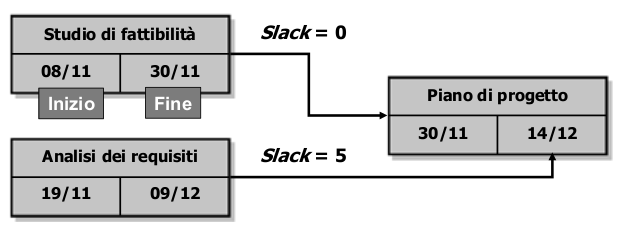
\includegraphics[scale=0.5]{images/8.png}\\
Per slack si intende il margine temporale tra due attività, ovviamente uno slack negativo non è possibile altrimenti vorrebbe dire che vado ad assegnare personale e risorse ad un'attività senza che l'input per tale attività sia pronto.}
\cornell{WBS}{Work Breakdown Structure\\
Ogni attività ha sottoattività non necessariamente sequenziale, ma comunque ben (univocamente) identificate\\
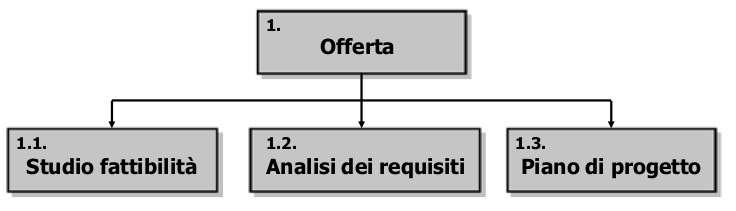
\includegraphics[scale=0.4]{images/9.png}}
\cornell{Problemi nell'allocazione delle risorse}{Bisogna fare attenzione ad evitare queste trappole durante l'assegnazione di risorse: \begin{itemize}
\item Sottostimare le necessità
\item Sovrastimarle
\end{itemize}}
\cornell{CoCoMo}{Constructive Cost Model\\
Essenzialmente una formula per valutare le risorse necessarie, esprimendole in mesi-persona. Crea una serie di stime che possono essere rappresentate come curve.}
\cornell{Piano di Progetto}{Documentazione letta da un verificatore, alcuni dati vanno condivisi con gli stakeholder e poi, una volta consolidato, viene visto dai membri del team.\\
Contiene scopo, organizzazione del progetto e soprattutto \underline{analisi dei rischi}}
\cornell{Rischi da Evitare}{\begin{itemize}
\item Sforamento dei Costi
\item Sforamento dei Tempi
\item Risultati insoddisfacenti
\end{itemize}}
\cornell{Fattori Di Fallimento}{\begin{itemize}
\item Requisiti Incompleti
\item Mancato coinvolgimento del cliente
\item Mancanza di Risorse
\item Fluttuazione dei requisiti
\end{itemize}}
\cornell{Fattori di Successo}{\begin{itemize}
\item Coinvolgimento Del Cliente
\item Verità riguardo alla disponibilità del personale
\item Definizione chiara dei requisiti
\end{itemize}}
